%@AUTHOR: Cardel
%Configuracion del documento

\documentclass{beamer}
\usetheme{Berkeley}
\setbeamertemplate{caption}[numbered]
\usepackage{graphicx}
\usepackage[utf8]{inputenc}
\usepackage[spanish]{babel}
\usepackage{ragged2e}
\usepackage{colortbl}
\usepackage{color}
\definecolor{naranja}{rgb}{1,0.5,0} % valores de las componentes roja, verde y azul (RGB)
\definecolor{rojo}{rgb}{1,0,0}
\definecolor{SteelBlue}{rgb}{0.3,0.5,0.7}
\usepackage{float}

\author{Carlos Andr\'es Delgado S.} 
\title{710193M Arquitectura de computadores II}
\subtitle{Aritmética del computador: Representación punto flotante \\ carlos.andres.delgado@correounivalle.edu.co}
\institute{Facultad de Ingeniería. Universidad del Valle}
%Transparencia
\setbeamercovered{transparent}

%LOGO Univalle
\pgfdeclareimage[height=1.4cm]{logo}{imagenes/univalle}
\logo{\pgfuseimage{logo}}

\usepackage{listings}% http://ctan.org/pkg/listings
\usepackage{listingsutf8}

\lstset{ %
  basicstyle=\footnotesize,           % the size of the fonts that are used for the code
  numbers=left,
  numberstyle=\footnotesize,          % the size of the fonts that are used for the line-numbers
  numbersep=4pt,                  % how far the line-numbers are from the code
  backgroundcolor=\color{white},      % choose the background color. You must add \usepackage{color}
  breaklines=true,                % sets automatic line breaking
  breakatwhitespace=true,        % sets if automatic breaks should only happen at whitespace
  title=\lstname,                   % show the filename of files included with \lstinputlisting;{}
  extendedchars=false,
  inputencoding=utf8, 
  tabsize=2,
   mathescape=true,
  literate={\ \ }{{\ }}1
}
\newsavebox{\myLst}
\newsavebox{\myLstb}
\newsavebox{\myLstc}
\newsavebox{\myLstd}


%Para que en cada seccion aparezca la tabla de contenido
\AtBeginSection[]{
	\begin{frame}
	\frametitle{Contenido}
	\tableofcontents[currentsection]
\end{frame}
}



\date{Febrero de 2016}
\newcommand{\grad}{\hspace{-2mm}$\phantom{a}^{\circ}$}
\begin{document}

\begin{frame}
	\titlepage	 		
\end{frame}

\begin{frame}
	\tableofcontents	 		
\end{frame}
\section{Representación en punto flotante}

\begin{frame}
	\frametitle{Representación en punto flotante}
	\begin{block}{Definiciones}
		\begin{itemize}
			\item En la representación complemento a dos es posible representar enteros positivos o negativos
			\item Sin embargo, no es posible representar números fraccionarios
			\item Se requiere un gran número de bits para representar números grandes
		\end{itemize}
	\end{block}	
\end{frame}

\begin{frame}
	\frametitle{Representación en punto flotante}
	\begin{block}{Definiciones}
		\begin{itemize}
			\item En el sistema decimal las anteriores limitaciones se superan usando notación científica:
			\begin{enumerate}
				\item $10000000000 = 1x10^{10}$
				\item $0.00000254 = 2.54x10^{-6}$
			\end{enumerate}
			\item Esta representación se utiliza para correr la coma decimal, tantas potencias de 10 se le indique. Si se corre la izquierda la potencia es positiva y si se corre a la derecha es potencia negativa.
		\end{itemize}
	\end{block}	
\end{frame}

\begin{frame}
	\frametitle{Representación en complemento a dos}
	\begin{block}{Ejercicio en clase}
	Transforme las siguientes expresiones en notación científica:
		\begin{itemize}
			\item $15200000000$
			\item $0.0000012445$
			\item $0.155457878454$
		\end{itemize}
	\end{block}	
\end{frame}

\begin{frame}
	\frametitle{Representación en complemento a dos}
	\begin{block}{Ejercicio en clase}
	Respuesta:
		\begin{itemize}
			\item $1,52x10^{10}$
			\item $1,2445x10^{-6}$
			\item $0.155457878454x10^{0}$
		\end{itemize}
	\end{block}	
	\begin{alertblock}{Limitaciones}
	Observe que no aplica para todos los casos, como es el caso de $0.155457878454$, no se puede acortar la representación utilizando notación científica de lo contrario se podría perder información.
	\end{alertblock}
\end{frame}

\begin{frame}
	\frametitle{Representación en punto flotante}
	\begin{block}{Definiciones}
		La técnica de notación científica se puede aplicar a los números binarios.
	\end{block}	
	\begin{block}{Notación científica binarios}
	\begin{equation}
		\pm S x B^{\pm E}
	\end{equation}
	
		\begin{enumerate}
			\item $\pm$ Signo
			\item $S$ Mantisa: Parte significativa
			\item $E$ Exponente
			\item $B$ Base, en binario es 2
		\end{enumerate}

	\end{block}
\end{frame}

\begin{frame}
	\frametitle{Representación en punto flotante}
	\begin{block}{Definiciones}
		\begin{enumerate}
			\item Si el bit MSB (más significativo) es 0, el n\'umero es positivo y si es 1, el n\'umero es negativo
			\item El exponente consta de 8 bits.
			\item Se utiliza \textbf{representación sesgada}
		\end{enumerate}
	\end{block}
\end{frame}

\begin{frame}
	\frametitle{Representación en punto flotante}
	\begin{block}{Representación sesgada}
		\begin{enumerate}
			\item Es un valor que se le resta al exponente
			\item Es denominado como \textbf{sesgo}
			\item Tiene un valor de $2^{k-1}-1$, $k$ es el número de bits del exponente
			\item Por lo que en un campo de 8 bits, este comprende entre un valor en el rango -127  a +128
		\end{enumerate}
	\end{block}
\end{frame}



\begin{frame}
	\frametitle{Representación en punto flotante}
	\begin{figure}[H]
	\centering
	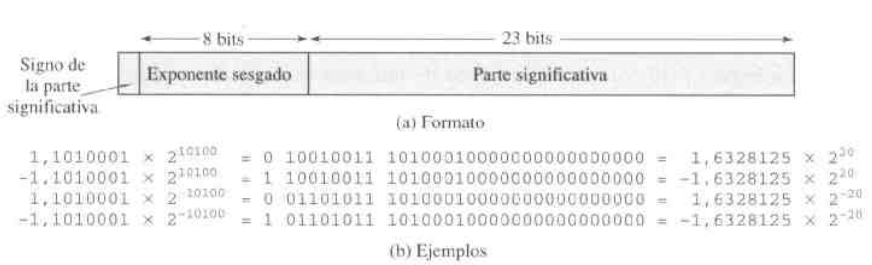
\includegraphics[scale=0.3]{imagenes/ejemplo.png}
	\caption{Formato típico de 32 bits en coma flotante}
	\end{figure}	
\end{frame}


\begin{frame}
	\frametitle{Representación en punto flotante}
	\begin{block}{Observaciones}
		\begin{enumerate}
			\item Las siguientes representaciones son equivalentes:\\
			$0,110*2^{5}$ \\
			$110*2^{2}$ \\
			$0,0110*2^{6}$ \\
			Para simplificarlos cálculos se utiliza la siguiente representación:\\
			$\pm 0.1bbbb * 2^{\pm E}$	
			\item Como se puede observar siempre tiene un 1 el el bit más a la izquierda
			\item Este bit se puede quitar y cuando se realizan los cálculos se vuelve a colocar
		\end{enumerate}
	\end{block}
\end{frame}


\begin{frame}
	\frametitle{Representación en punto flotante}
	\begin{block}{Observaciones}
		Por lo que este formato:
		\begin{enumerate}
			\item El signo se almacena en el bit más a la izquierda
			\item El primer bit de la parte significativa siempre es 1, por lo que puede quitarse
			\item Se suma 127 al exponente original
			\item La base es 2
		\end{enumerate}
	\end{block}
\end{frame}


\begin{frame}
	\frametitle{Complemento a dos vs representación en punto flotante}
	\begin{figure}[H]
	\centering
	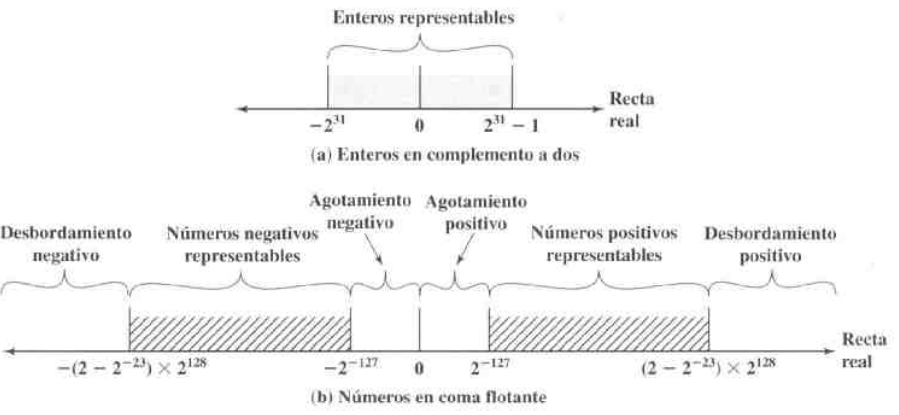
\includegraphics[scale=0.3]{imagenes/complementoa2puntoflotante.png}
	\caption{Comparación representación a dos vs punto flotante}
	\end{figure}	
\end{frame}

\begin{frame}
	\frametitle{Representación en punto flotante}
	\begin{block}{Rango}
		Para el formato de representación en punto flotante se tienen los siguientes rangos:
		\begin{enumerate}
			\item Números negativos entre $-(2 - 2^{23}) * 2^{128}$ y $-2^{-127}$
			\item Números positivos entre $-2^{-127}$ y $(2 - 2^{23}) x 2^{128}$ 
		\end{enumerate}
	\end{block}
\end{frame}


\begin{frame}
	\frametitle{Representación en punto flotante}
	\begin{block}{Regiones}
	   En la recta se pueden observar las siguientes regiones se encuentran excluidas:
		\begin{enumerate}
			\item \textbf{Desbordamiento negativo:} números negativos menores que: $-(2 - 2^{23}) x 2^{128}$
			\item \textbf{Agotamiento negativo:} números negativos mayores que: $-2^{-127}$
			\item \textbf{Agotamiento positivo:} números positivos menores $2^{-127}$ 
			\item \textbf{Desbordamiento positivo:} números positivos mayores que $(2 - 2^{23}) x 2^{128}$ 
			\item El zero
		\end{enumerate}
	\end{block}
\end{frame}

\begin{frame}
	\frametitle{Representación en punto flotante}
	\begin{block}{Densidad}
	Se puede observar que el espaciamiento entre los números en coma flotante no es uniforme:	
	\begin{figure}[H]
		\centering
		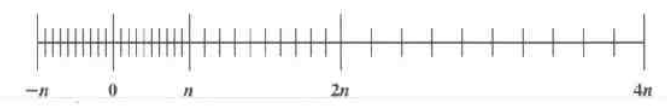
\includegraphics[scale=0.3]{imagenes/densidad.png}
		\caption{Densidad de los números en coma flotante}
	\end{figure}
	Se puede observar que existe una gran población de números cerca al origen
	\end{block}
\end{frame}


\section{Estándar del IEEE para punto flotante}
\begin{frame}
	\frametitle{Estándar del IEEE para punto flotante}
	\begin{block}{Formatos}
		\begin{enumerate}
			\item \textbf{Formato simple:} 32 bits
			\item \textbf{Formato doble:} 64 bits
		\end{enumerate}
	\begin{figure}[H]
		\centering
		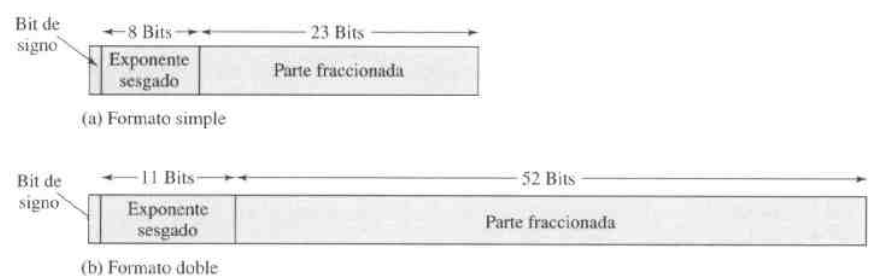
\includegraphics[scale=0.3]{imagenes/ieee754.png}
		\caption{Formatos IEEE 754}
	\end{figure}
	\end{block}
\end{frame}

\begin{frame}
	\frametitle{Estándar del IEEE para punto flotante}
	\begin{block}{Formatos}
		\begin{enumerate}
			\item \textbf{Formato simple:} 32 bits
			\item \textbf{Formato doble:} 64 bits
		\end{enumerate}
	\begin{figure}[H]
		\centering
		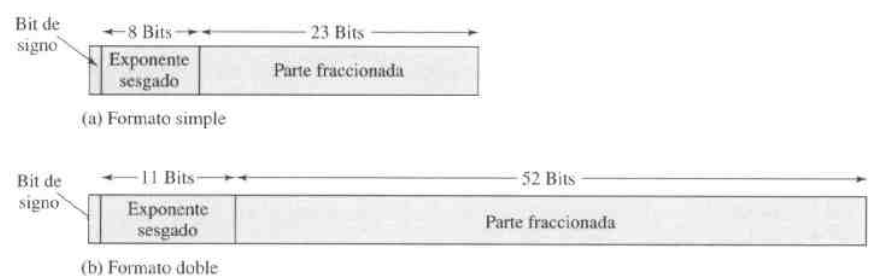
\includegraphics[scale=0.3]{imagenes/ieee754.png}
		\caption{Formatos IEEE 754}
	\end{figure}
	\end{block}
\end{frame}

\begin{frame}
	\frametitle{Estándar del IEEE para punto flotante}
	\begin{figure}[H]
		\centering
		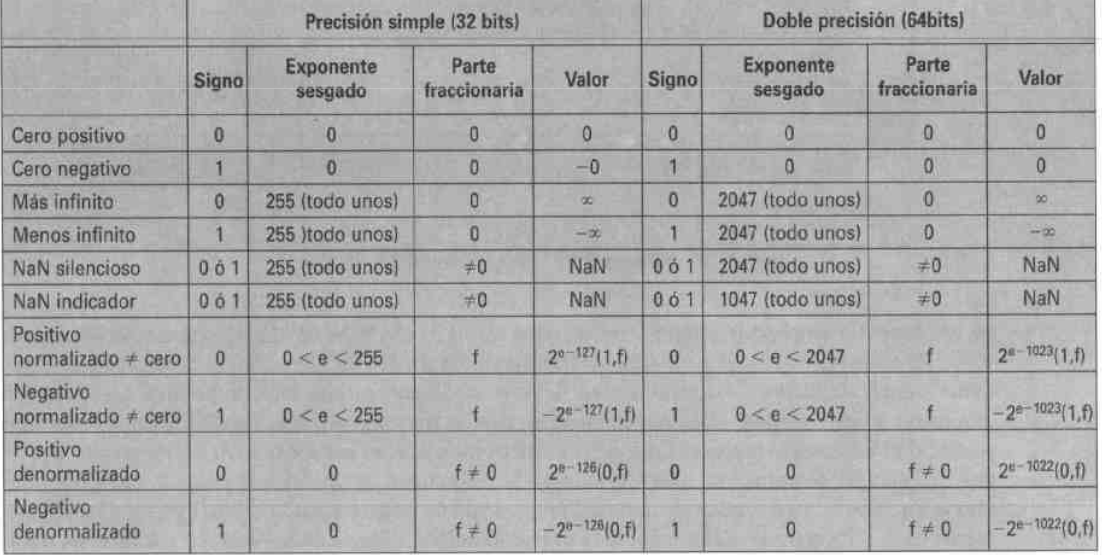
\includegraphics[scale=0.25]{imagenes/valoresespecialesIEEE754.png}
		\caption{Interpretación números en coma flotante}
	\end{figure}
\end{frame}

\begin{frame}
	\frametitle{Estándar del IEEE para punto flotante}
	\begin{block}{Ejemplos}
	Transforme al estándar IEEE 754 de 32 bits los siguientes números:
	\begin{enumerate}
		\item $10.5_{10}$
		\item $17236_{10}$
		\item $-127.125_{10}$
	\end{enumerate}	
	\end{block}
\end{frame}

\begin{frame}
	\frametitle{Estándar del IEEE para punto flotante}
	\begin{block}{Ejemplos}
	\textbf{Paso 1:} Transforme el número en binario
	\begin{enumerate}
		\item $1010.1_{2}$
		\item $100001101010100_{2}$
		\item (Signo negativo) $1111111.001_{2}$
	\end{enumerate}	
	\end{block}
\end{frame}


\begin{frame}
	\frametitle{Estándar del IEEE para punto flotante}
	\begin{block}{Ejemplos}
	\textbf{Paso 2:} Normalice el número
	\begin{enumerate}
		\item $1.0101_{2}*(10^{3})_{2}$
		\item $1.00001101010100_{2}*(10^{14})_{2}$
		\item (Signo negativo) $1.111111001_{2}*(10^{6})_{2}$
	\end{enumerate}	
	\end{block}
\end{frame}


\begin{frame}
	\frametitle{Estándar del IEEE para punto flotante}
	\begin{block}{Ejemplos}
	\textbf{Paso 3:} Calcula el exponente, recuerda que para el caso de 32 bits, el sesgo es $2^8 - 1$ entonces es $127_{10}=1111111_{2}$
	\begin{enumerate}
		\item $127_{10}+3_{10} = 130_{10} = 10000010_{2}$
		\item $127_{10}+14_{10} = 141_{10} = 10001101_{2}$
		\item (Signo negativo) $127_{10}+6_{10} = 133_{10} = 10000101_{2}$
	\end{enumerate}	
	\end{block}
\end{frame}

\begin{frame}
	\frametitle{Estándar del IEEE para punto flotante}
	\begin{block}{Ejemplos}
	\textbf{Paso 4:} Se obtiene el número en estándar IEEE 754 de 32 bits:
		\begin{table}[H]
		\begin{tabular}{|c|c|c|}
		\hline 
		\textbf{Signo} & \textbf{Exponente }& \textbf{Mantisa} \\ 
		\hline 
		0 & 10000010 & \textbf{0101}0000000000000000000000000000 \\ 
		\hline 
		0 & 10001101 & \textbf{00001101010100}000000000000000000 \\ 
		\hline 
		1 & 10000101 & \textbf{111111001}00000000000000000000000 \\ 
		\hline 
		\end{tabular}
		\end{table} 
	\end{block}
	Verifiquemos:\\ \url{http://www.h-schmidt.net/FloatConverter/IEEE754.html} Consultado Feb 2016
\end{frame}

\begin{frame}
	\frametitle{Estándar del IEEE para punto flotante}
	\begin{block}{Ejercicio en clase}
	Transforme al estándar IEEE 754 de 32 bits los siguientes números:
	\begin{enumerate}
		\item $18.75_{10} = 10010.11_{2}$
		\item $14578.5_{10} = 11100011110010.1_{2} $
		\item $-0.625_{10} = 0.101_{2}$
	\end{enumerate}	
	\end{block}
\end{frame}


\begin{frame}
	\frametitle{Estándar del IEEE para punto flotante}
	\begin{block}{Ejercicio en clase}
	Respuestas:
	\begin{enumerate}
		\item $01000001100101100000000000000000_{2}$
		\item $01000110011000111100101000000000_{2}$
		\item $10111111001000000000000000000000_{2}$
	\end{enumerate}	
	\end{block}
\end{frame}

\begin{frame}
	\frametitle{Estándar del IEEE para punto flotante}
	\begin{block}{Ejercicio en clase}
	Ahora intenta para 64 bits, recuerda: exponente 11 bits y mantisa 53 bits.
	\begin{enumerate}
		\item $18.75_{10} = 10010.11_{2}$
		\item $14578.5_{10} = 11100011110010.1_{2} $
		\item $-0.625_{10} = 0.101_{2}$
	\end{enumerate}	
	\end{block}	
	\begin{center}
	\textbf{¿Cuanto es el sesgo?}
	\\Recuerda es: $2^{k-1}-1$, donde $k$ es el número de bits del exponente
	\end{center}
	\end{frame}

\begin{frame}
	\frametitle{Estándar del IEEE para punto flotante}
	\begin{block}{Ejercicio en clase}
	Respuestas:
	\scriptsize{
	\begin{enumerate}
		\item $0100000000110010110000000000000000000000000000000000000000000000_{2}$
		\item $0100000011001100011110010100000000000000000000000000000000000000_{2}$
		\item $1011111111100100000000000000000000000000000000000000000000000000_{2}$
	\end{enumerate}
	}	
	\end{block}
\end{frame}

\begin{frame}
	\frametitle{Estándar del IEEE para punto flotante}
	\begin{block}{Ejemplos}
	Transforme a decimal los siguientes números en el estándar IEEE 754 de 32 bits:
	\begin{enumerate}
		\item $01000001001100000000000000000000_{2}$
		\item $11000000110100000000000000000000_{2}$
		\item $01000010010010000000000000000000_{2}$
	\end{enumerate}	
	\end{block}
\end{frame}

\begin{frame}
	\frametitle{Estándar del IEEE para punto flotante}
	\begin{block}{Ejemplos}
	\textbf{Paso 1}: Reste el sesgo al exponente
	\begin{enumerate}
		\item $10000010_{2} - 1111111_{2}$
		\begin{itemize}
			\item $130_{10} - 127_{10}$
			\item $3_{10}$
		\end{itemize}
		\item $10000001_{2} - 1111111_{2}$
		\begin{itemize}
			\item $129_{10} - 127_{10}$
			\item $2_{10}$
		\end{itemize}
		\item $10000100_{2} - 1111111_{2}$
		\begin{itemize}
			\item $132_{10} - 127_{10}$
			\item $5_{10}$
		\end{itemize}
	\end{enumerate}	
	\end{block}
\end{frame}

\begin{frame}
	\frametitle{Estándar del IEEE para punto flotante}
	\begin{block}{Ejemplos}
	\textbf{Paso 2}: Agregue $1.$ a la mantisa
	\begin{enumerate}
		\item $1.01100000000000000000000_{2}$
		\item $1.10100000000000000000000_{2}$
		\item $1.10010000000000000000000_{2}$
	\end{enumerate}	
	\end{block}
\end{frame}

\begin{frame}
	\frametitle{Estándar del IEEE para punto flotante}
	\begin{block}{Ejemplos}
	\textbf{Paso 3}: Multiplique por $2$ elevado al exponente al que se le ha restado el sesgo
	\begin{enumerate}
		\item $1.01100000000000000000000_{2}*2^{3}$
		\item $1.10100000000000000000000_{2}*2^{2}$
		\item $1.10010000000000000000000_{2}*2^{5}$
	\end{enumerate}
		En binario, multiplicar por 2 es análogo a multiplicar por 10 en decimal, \textbf{sólo debes correr la coma tantas posiciones a la derecha o izquierda}
		
	\end{block}
\end{frame}

\begin{frame}
	\frametitle{Estándar del IEEE para punto flotante}
	\begin{block}{Ejemplos}
	\textbf{Paso 4}: Convierta en decimal, tome en cuenta el bit del signo
	\begin{enumerate}
		\item $1011.00000000000000000000_{2}=11_{10}$
		\item $-110.100000000000000000000_{2}=-6.5_{10}$
		\item $110010.000000000000000000_{2}=-50_{10}$
	\end{enumerate}		
	\end{block}
\end{frame}

\begin{frame}
	\frametitle{Estándar del IEEE para punto flotante}
	\begin{block}{Ejercicio}
	Transforme a decimal los siguientes números en el estándar IEEE 754 de 32 bits:
	\begin{enumerate}
		\item $01000010000001010000000000000000_{2}$
		\item $11000001011110000000000000000000_{2}$
		\item $01000010110010001000000000000000_{2}$
	\end{enumerate}	
	\end{block}
\end{frame}

\begin{frame}
	\frametitle{Estándar del IEEE para punto flotante}
	\begin{block}{Ejercicio}
	Respuestas:
	\begin{enumerate}
		\item $33.25_{10}$
		\item $-15.5_{10}$
		\item $100.25_{10}$
	\end{enumerate}	
	\end{block}
\end{frame}

\section{Aritmética en punto flotante}

\begin{frame}
	\frametitle{Aritmética en punto flotante}
	\begin{block}{Definiciones}
	\begin{itemize}
		\item Sumas y restas más complicadas que la multiplicación y división, imagine que tiene que sumar $3*10^{5}+4*10^{3}$.
		\item Por lo tanto, para sumas y restas es necesario ajustar el exponente.
	\end{itemize}	
	\end{block}
\end{frame}

\begin{frame}
	\frametitle{Aritmética en punto flotante}
	\begin{block}{Sumas y restas}
	Se deben realizar 4 pasos:
	\begin{enumerate}
		\item \textbf{Comprobación de cero:} Debido a que la suma y la resta son idénticas, excepto por el cambio de signo, en el caso de restas se cambia el signo del \textbf{substraendo}
		\item \textbf{Ajuste cifras significativas:} Ajuste el menor exponente igual al mayor exponente, realizando los corrimientos de coma necesarios:\\
		$123*10^0 + 456*10^{-2} = 123*10^0 + 4.56*10^{0} = 127.56*10^{0}$
		\item \textbf{Realice la suma respectiva, tomando en cuenta el signo de los operandos}
		\item Normalización, recuerde que la mantisa tiene forma $1.bbbb$
	\end{enumerate}	
	\end{block}
\end{frame}

\begin{frame}
	\frametitle{Aritmética en punto flotante}
	\begin{block}{Ejemplo 1}
	Realice la siguiente operación:
	\begin{enumerate}
		\item $01000010100101010000000000000000_{2} + 01000000011100000000000000000000_{2}$ 
		\\ $74.5_{10} + 3.75_{10}$
	\end{enumerate}	
	\end{block}
\end{frame}

\begin{frame}
	\frametitle{Aritmética en punto flotante}
	\begin{block}{Ejemplo 1}
	\textbf{Paso 1: Comprobación de cero:}
	\begin{enumerate}
		\item $01000010100101010000000000000000_{2} + 01000000011100000000000000000000_{2}$ 
	\end{enumerate}	
	En este caso ya que los dos son positivos y se trata de una suma, no se realiza ningún cambio de signo
	\end{block}
\end{frame}

\begin{frame}
	\frametitle{Aritmética en punto flotante}
	\begin{block}{Ejemplo 1}
	\textbf{Paso 2: Ajuste cifras significativas:}
		\begin{itemize}
			\item Exponentes: $10000101_{2}, 10000000_{2}$ 
			\item Mantisas: $1.00101010000000000000000_{2},1.11100000000000000000000_{2}$
			\item La diferencia entre los exponentes es: $101_{2} = 5_{10}$ por lo que se deben correr $5$ posiciones a la izquierda la segunda mantisa así:
			\\ Mantisas: $1.00101010000000000000000_{2}$,\\\textbf{$0.0000111100000000000000000000_{2}$}
		\end{itemize}		
	\end{block}
\end{frame}



\begin{frame}
	\frametitle{Aritmética en punto flotante}
	\begin{block}{Ejemplo 1}
	\textbf{Paso 3: Suma:}
		Mantisas normalizadas: \\ $1.00101010000000000000000_{2}$,\\\textbf{$0.0000111100000000000000000000_{2}$}
		\begin{itemize}
			\item Se realiza la suma de las mantisas para obtener:\\
			$1.00111001000000000000000_{2}$
			\item Como en este caso ha quedado de la forma $1.0$ no es necesario cambiar el exponente.
			\item Por lo que el resultado es: $0 10000101 00111001000000000000000_{2} = 78.25_{10}$.							
		\end{itemize}		
	\end{block}
\end{frame}



\begin{frame}
	\frametitle{Aritmética en punto flotante}
	\begin{block}{Ejemplo 2}
	Realice la siguiente operación:
	\begin{enumerate}
		\item $11000001110011000000000000000000_{2} - 01000001100011100000000000000000_{2}$
		\\ $-25.5_{10} - 17.75_{10}$
	\end{enumerate}	
	\end{block}
\end{frame}

\begin{frame}
	\frametitle{Aritmética en punto flotante}
	\begin{block}{Ejemplo 2}
	\textbf{Paso 1: Comprobación de cero:}
	\begin{enumerate}
		\item $11000001110011000000000000000000_{2} + 11000001100011100000000000000000_{2}$
	\end{enumerate}	
	En este caso se tiene una resta por lo que el \textbf{substraendo} se cambia de signo.
	\end{block}
\end{frame}


\begin{frame}
	\frametitle{Aritmética en punto flotante}
	\begin{block}{Ejemplo 2}
	\textbf{Paso 2: Ajuste cifras significativas:}
		\begin{itemize}
			\item Exponentes: $10000011_{2}, 10000011_{2}$ 
			\item Mantisas: $1.10011000000000000000000_{2}$,\\$1.00011100000000000000000_{2}$
			\item Como se puede observar ambos exponentes son iguales, por lo que no se realizan cambios en las mantisas.
		\end{itemize}		
	\end{block}
\end{frame}


\begin{frame}
	\frametitle{Aritmética en punto flotante}
	\begin{block}{Ejemplo 2}
	textbf{Paso 3: Suma:}
		Mantisas: $1.10011000000000000000000_{2}$,\\$1.00011100000000000000000_{2}$
		\begin{itemize}
			\item Como son ambos negativos, se suma sin problema y se toma en cuenta que el resultado es negativo
			\item El resultado de la suma es: $10.10110100000000000000000_{2}$
			\item Como en este caso no ha quedado de la forma $1.0$ es necesario correr la coma una posición a la izquierda, \textbf{que es equivalente a sumar 1 al exponente} y la mantisa ahora es: $1.01011010000000000000000$ \textbf{0} $_{2}$
			\item Por lo que el nuevo exponente es: $10000100_{2}$
			\item El resultado total es: $1 10000100 01011010000000000000000_{2} = -43.25_{10}$.
		\end{itemize}		
	\end{block}
\end{frame}




\begin{frame}
	\frametitle{Aritmética en punto flotante}
	\begin{block}{Multiplicación y división}
	\begin{itemize}
		\item Para el caso de multiplicación, se suman los exponentes, pero a uno de ellos se le debe restar el sesgo, de lo contrario lo está sumando 2 veces. En el caso de la división se realiza la resta y se le suma el sesgo.
		\item Las mantisas se multiplican o dividen segundo el caso
		\item Considere los signos y aplique la \textbf{ley de los signos} según el caso
	\end{itemize}	
	\end{block}
\end{frame}

\begin{frame}
	\frametitle{Aritmética en punto flotante}
	\begin{block}{Ejemplo}
	Realice las siguientes multiplicaciones y divisiones:
	\begin{enumerate}
		\item $01000001100000000000000000000000_{2} + 01000000001000000000000000000000_{2}$ 
		\\ $16_{10} * 2.5_{10}$
		\item $01000001100000000000000000000000_{2} - 01000000100000000000000000000000_{2}$
		\\ $16_{10} / 4_{10}$
	\end{enumerate}	
	\end{block}
\end{frame}

\begin{frame}
	\frametitle{Aritmética en punto flotante}
	\begin{block}{Ejemplo}
	Ajuste exponentes:
	\begin{enumerate}
		\item $0 10000011 00000000000000000000000_{2} + 0 10000000 01000000000000000000000_{2}$ 
		\\ $10000011_{2} + 10000000_{2} - 1111111_{2} = 10000100_{2}$
		\item $0 10000011 00000000000000000000000_{2} - 0 10000001 00000000000000000000000_{2}$
		\\ $10000011_{2} - 10000001_{2} + 1111111_{2} = 10000001_{2}$
	\end{enumerate}	
	\end{block}
\end{frame}

\begin{frame}
	\frametitle{Aritmética en punto flotante}
	\begin{block}{Ejemplo}
	Ajuste mantisas:
	\begin{enumerate}
		\item $0 10000011 00000000000000000000000_{2} + 0 10000000 01000000000000000000000_{2}$ 
		\\ $1.00000000000000000000000_{2} * 1.01000000000000000000000 = 1.01000000000000000000000_{2}$
		\item $0 10000011 00000000000000000000000_{2} - 0 10000001 00000000000000000000000_{2}$
		\\ $1.00000000000000000000000_{2} / 1.00000000000000000000000 = 1.00000000000000000000000_{2}$
	\end{enumerate}	
	\end{block}
\end{frame}

\begin{frame}
	\frametitle{Aritmética en punto flotante}
	\begin{block}{Ejemplo}
	Uniendo resultados:
	\begin{enumerate}
		\item $0 10000100 01000000000000000000000_{2} = 40_{10}$ 
		\item $0 10000001 00000000000000000000000_{2} = 4_{10}$
	\end{enumerate}	
	\end{block}
\end{frame}

\begin{frame}
	\frametitle{Preguntas}
	\vfill
	\begin{center}
	¿Preguntas?\\
	\vfill
	Siguiente clase: \\
	Repertorio de Instrucciones: \\
	Características y funciones
	\end{center}
\end{frame}



\end{document}